\documentclass[11pt,a4paper]{article}
\usepackage[utf8]{inputenc}
\usepackage[T1]{fontenc}
\usepackage{amsmath}
\usepackage{amsfonts}
\usepackage{amssymb}
\usepackage{graphicx}
\usepackage[left=2.00cm, right=2.00cm, top=2.00cm, bottom=2.00cm]{geometry}
\usepackage{tikz}
\usetikzlibrary{arrows.meta, automata, shapes, arrows, calc, positioning, quotes}
\tikzstyle{dfa} = [rectangle, rounded corners, minimum width=3cm, minimum height=1cm,text centered, text=white, fill=blue!100, text width = 6.5cm]
\tikzstyle{nn} = [rectangle,  rounded corners, minimum width=3cm, minimum height=1cm,text centered, text=white, fill=red!100, text width = 6cm]
\tikzstyle{process} = [trapezium, trapezium left angle=70, trapezium right angle=110, minimum width=3cm, minimum height=0.5cm, text centered, draw=black, fill=gray!30, inner xsep=0pt,outer sep=0pt]
\tikzstyle{comparison} = [diamond, text centered, draw=black, fill=green!50, /pgf/aspect=1.3]
\tikzset{
	FARROW/.style={line width=2pt, arrows={-Latex[angle=40:4mm]}}
}
\tikzstyle{arrow} = [thick,->,>=stealth]
\usepackage{url,hyperref}
\begin{document}
	
	
	\section*{Overview}
	
		In the summer 1951, the great American mathematician Stephen Kleene developed the fundamental notion of \emph{regular expression} to describe the class of events leading to a given state in a finite automaton ~\cite[Theorem 6]{kleene1951}. The latter is explicitly understood in \textit{op.cit.}\ as an abstraction and generalisation of a McCulloch-Pitts nerve net, a logical model of nervous activity which we would today describe as a kind of \emph{neural network}. The theory of automata, one of the pillars of formal methods in computer science, was thus born out of a desire to understand neural networks. The key role of Kleene's approach and motivation is reflected by the presence of a version of \textit{op.cit.}\ as the very first chapter of the 1956 \textit{Automata Studies}~\cite{ashby1956automata}, the volume that cemented automata theory as a discipline, along contributions from von Neumann, Shannon, Moore, Minsky, etc. 
		
		Automata and neural network theory have since followed diverging paths, leading to the establishment of largely disjoint research communities. Interestingly though, both of these paths have lead to the development of important supervised learning paradigms implemented by well-known algorithms ($L^\ast$ and stochastic gradient descent respectively). 		
		This project aims to rekindle the connection between automata and neural networks, and specifically to explore how these two learning paradigms can help improve and explain each other.
		Concretely, the project is structured around  three complementary axes:
		\begin{enumerate}
			\item Using deep neural networks to improve automaton learning.
			\item Using automata to improve deep neural network learning.
			\item Using automata to improve our understanding of deep neural network mechanisms and behaviours.
		\end{enumerate}
		The first two axes combine into the development of an ecosystem of concrete and practical techniques to assist in one type of learning by applying idea from the other. 
		As we will see, this ecosystem could allow us to create learning systems \emph{combining features of both automaton and deep neural network learning}, for instance machine learning systems guided by formal automata-theoretic constraints who are themselves learned with the help of Neural Networks. 
	
	The last axis has a more fundamental and theoretical ambition: to use automata as a highly structured class of classification problems with which to investigate whether \emph{logical and compositional reasoning} can be (a) identified and (b) understood in various deep neural network architectures.
	
	\section*{WP1: Improving Automaton Learning with deep neural networks}
	\emph{Finite automata} are perhaps the simplest and best-understood model of computation. A finite automaton represents a simple `computing machine' which runs programs written in a very simple `programming language' called a regular expression. An automaton can thus be seen as a classification algorithm deciding whether a given program belongs to such a language or not: simply feed the program to the automaton and check whether it executes successfully or not. Finite automata and variations thereof and not only theoretically important, they also model a huge variety of systems of practical interest in computer science such as networks, decision processes, etc.
	
	In 1987 Dana Angluin developed the now famous $L^\ast$-algorithm~\cite{angluin1987learning} which showed that it is possible to \emph{learn an unknown automaton} by $(i)$ feeding it programs and observing whether they run successfully or not (these interactions are called membership queries), and $(ii)$ asking for a counter-example program that runs successfully on the algorithm's current representation of the unknown automaton, but not on the actual unknown automaton (these interactions are called equivalence queries).  The Cornell pole of the project has unrivalled expertise in applying and extending this algorithm to an extremely wide variety of contexts, e.g.\ learning nominal automata~\cite{moerman2017learning}, tree-automaton~\cite{heerdt2022categorical}, automata for concurrent processes ~\cite{van2021learning}, automata with side-effects~\cite{van2020learning} and apply it to important concrete applications to e.g.\ network verification~\cite{ferreira2021prognosis}.
	  
	There are two practical obstacles to Angluin's algorithm that we believe deep neural networks could alleviate: (1) counter-example generation and (2) scope and scale.
	\setcounter{section}{1}
	\setcounter{subsection}{0}
		\subsection{Counter-example generation}
		A major practical obstacle in Angluin's algorithm is that of implementing equivalence queries since, by definition, the target automaton is unknown. Counter-examples are typically generated by exhaustive testing, which is highly resource and time-intensive particularly in physical systems such as networks. To solve this problem, we propose that the  QMUL pole develop and train neural networks architectures to generate counter-examples in Angluin's learning algorithm. The following strategies will be investigated
		\begin{itemize}
			\item Use the strings which fail membership queries (and are discarded by Angluin's algorithm) to train a Generative Adversarial Network (GAN) to produce counter-examples.
			\item Use the strings which fail membership queries to train a transformer architecture to produce counter-examples (using the alphabet of the automaton as tokens).
			\item Train a classifier using both positive and negative membership queries in parallel to the $L^\ast$-algorithm and use this classifier as the basis for a generative model able to produce counter-examples when required (there are several techniques to do this \cite{?}).
		\end{itemize}
		
		
		\subsection{Enlarging the scope of automata learning with NN adaptors}
		Another limitation in applying Angluin's algorithm or variants thereof is that at least one of the following problems frequently happens:
		\begin{itemize}
			\item[(i)] \emph{Scale}: the set of instructions which can be submitted to the unknown automaton -- often known as the System Under Learning or SUL -- is extremely large. As a concrete example, consider the case of an unknown network protocol which we are trying to learn. Instructions are packets and the set of possible packets is extremely and unnecessarily large. It is often possible to learn the protocol using a much smaller set of `abstract packets'.
			\item[(ii)] \emph{Scope}: the SUL is not quite a learnable automaton-like structure, but by abstracting away some of the features it is possible to understand the part of the system that behaves like an automaton. For a very simple example, consider a Mealy machine, that is to say a automaton which expects an input at each step of the computation. We may want to learn it's automaton behaviour under the assumption that it receives some abstract input (i.e.\ any input) at each step by abstracting the set of possible inputs to a singleton input (as it turns out it is possible to learn an Mealy machines as well \cite{}).
		\end{itemize}
		
		In both of these instances, learning the unknown system will require the ability to submit coarse-grained abstract queries to the SUL; that is to say queries where either part of the set of instructions or parts of the behaviour (or both) are abstracted away. 
		
		For the SUL to understand these abstract instructions and reply to a membership query, the abstract query must be `concretised' into a query that the SUL can understand.  As an example, suppose we wish to learn a network protocol which does not depend on the exact destination of a packet, but only on whether the destination is inside or outside a sub-network (e.g.\ an organisation). We then want to provide the SUL with abstract packets where the destination field is just a boolean flag. However, for the system to process such a packet it must be concretised and the destination field must be populated by some acceptable value.
		
		The mechanism that performs with concretisation, i.e.\ that transforms abstract instructions into concrete ones and vice-versa is called an Adapter \cite{ferreira2021prognosis} (ANY GENERAL REFERENCE ON THIS CONCEPT?). The abstraction part of the Adapter is usually user defined, easy to implement and very quick to evaluate. On the other hand, concretising abstract instructions amounts to \emph{non-deterministically generating} instructions along the inverse of the abstraction function. This task is moreover often context-dependent, that is to say each concretisation is usually dependent on previous concretisations, which greatly complicates the problem. 
		
		The non-trivial part of the adpater is currently solved by hand in an ad-hoc way (see e.g.\ \cite{ferreira2021prognosis}). This means in particular that many problems which could \emph{in principle} be solved by automaton learning, currently can't be because designing the required adapter by hand is too hard or time-consuming.
		
		We propose using deep neural networks to \emph{learn} adapters since this is exactly the kind of task that machine-learning algorithms such as next token prediction or sequence-to-sequence translation (Seq2Seq) with transformer architectures are very good at. 
		
		In this project we aim to develop a methodology for learning arbitrary adapters, investigate the most successful architectures for adapters, and whether general purpose adapters can be designed and then specialised to specific tasks by fine-tuning. With these very new machine-learned adapters we should be able to use automaton-learning to verify concrete implementations of complex network protocols such as XXX which are currently beyond the reach of state-of-the-art automaton learning techniques. OTHER EXAMPLES??
		
		
	\section*{WP2: Improving Neural Network Learning with Automata}
	Deep neural networks are by far the most successful learning paradigm in computer science, but in some instances it is desirable to combine their general-purpose but opaque solutions with expert knowledge or formal specifications in order to guarantee correctness or enforce certain formally specified behaviours. Techniques to achieve this difficult union fall under the umbrella of \emph{neurosymbolic AI}. In this work-package we propose to develop neursymbolic methods whose symbolic part is derived specifically from the theory of automata and automaton-learning.
	
	This work package is split into two components, the first one will be looking at enforcing regular-expression-like specifications by constructing new types of cost functions for neural-network training. This should therefore find applications in many type of neural-network architectures. The second work package will be looking more specifically at how these formal constraints can be enforced in the particular case of the transformer architecture behind the success of modern LLMs. Our ambition is to create a template for architectures designed to learn \emph{formal} languages, particularly in the absence of vast amounts of training data.
	
	\setcounter{section}{2}
	\setcounter{subsection}{0}
		\subsection{Automata-based cost functions}
			The idea of using automata to build cost functions has been explored in \cite{icarte2022reward} in the context of reinforcement learning. In this context, a (coarse-grained! connection with adaptors!) policy is described as a finite automaton together with a reward function for every transition.  
			We believe this idea could be generalised in two directions in the context of this project.
			\begin{enumerate}
				\item First, in terms of applicability. We propose investigating how the idea of constructing a cost/utility function out of a formal specification described by automata-like structures can be used in the context of LLM for code generation. Regular expressions, and variants thereof, are the ideal testing groud for testing this idea as they form what is arguably the simplest non-trivial example of formal/programming language. The idea would be to investigate if objective functions which penalise incorrect syntax encoded as automaton can be used to in the training of LLMs designed to generate regexes.
				\item Second, in terms of mathematics. Automata-based cost functions, reward-machines in the terminology of \cite{icarte2022reward}, are very ad-hoc constructions. Are there general constructions which can turn an automaton, of generalisation thereof, into an objective function? Ideally such a function would come with certain guarantees, for example being convex. Is this possible? And how can these function be combined to reflect the various ways in which automata can be combined? In other words, is there a compositional approach to `reward machines'?
			\end{enumerate} 
		
			Mention notions of distance between terms etc. (Work by Fred and Wojtek)
			
		\subsection{Towards Large \emph{Formal} Language Models (LFLMs): the case of regular expressions}
			Beyond the idea of automata-based cost functions. We plan to investigate the possibility of enforcing correct syntax into LLM by researching ways in which syntax can enforce the choice of the various blocks of a transformer stack. Specifically, looking at the case of regular expressions as the simplest non-trivial example of formal language: 
			\begin{enumerate}
				\item Embeddings: what is a sensible choice of dimensionality for the embedding of a tokens which might be few in numbers but combine in very specific ways. Are the constraints of a low-dimensional embedding helpful in this context or not? Does the size of the minimal automaton recognising a regex give any information about the dimensionality of good embeddings? By extending experiments along these lines to increasingly complex types of grammars/automata we might gain some understanding of what makes a good embedding for the ask of LFLM (Large Formal Language Model)
				\item Attention mechanism: can we design constrained attention mechanisms guided by automata?
			\end{enumerate}
		
		\subsection{Combining WP1 and WP2}
	
	\section*{WP3: Investigating logical and compositional reasoning in deep neural networks with automata}
	Explainable AI is a very active field of research but much remains mysterious about neural networks. How can we explain their incredible effectiveness versus other models of computation? Is it possible to understand how a neural network works -- and therefore also how it doesn't -- in a structural and compositional way, that is to say by understanding it as a composition of smaller and better understood sub-systems? Since these models find applications in virtually every industry, and will more or less directly impact everyone on the planet, these are societally crucial problems. 
	
	To investigate these questions we propose to use the expertise of the Cornell pole in the theory and industrial applications of \emph{finite automata}, one of the simplest and best-understood models of computations. A finite automaton represents a simple `computing machine' which can only successfully run programs written in a simple `programming language' called a regular expression. An automaton can thus be used to solve the problem of deciding whether a program belongs to such a language or not: simply feed the program to the automaton and check whether executes successfully or not. Neural networks can also solve this classification problem, and our proposal is therefore to use finite automata as a well-understood, well-behaved and sufficiently complex benchmarking and testing suite with which to probe the inner workings of neural networks. 
	
	
	This is not a new idea, \cite{cleeremans1989finite} provides a brief but very instructive example of this line of research from a natural language processing perspective. Much of the research at the intersection between neural network and finite automata has since focused on describing the behaviour of an unknown neural network as a finite automaton \cite{weiss2018extracting,weiss2019learning} or using automata theory to describe the computational power of neural networks \cite{weiss2018practical}. Our proposed approach combines the original idea of~\cite{cleeremans1989finite} -- trying to understand how a neural network works by discovering how it internally represents the finite automaton problem it is solving -- to the more recent work of \cite{weiss2018extracting,weiss2019learning} which which gives concrete algorithms to extract this internal representation. This will allow us to perform the following type of neural network probing experiment: (a) set an automaton problem, (b) solve it with a neural network, (c) extract the network's internal representation of the automaton, and (d) compare it to the original, as described in Figure \ref{diag:strategy}. 
	
	
	Finite automata form a space of problems with a rich inner structure, for example automata $A$ and $B$ can be combined in various ways to form new automata, say $A+B$. Using the strategy of Figure~\ref{diag:strategy} we can study the compositional nature of neural networks by understanding how the internal representations of $A$ and $B$ are combined to form an internal representation of $A+B$ in the neural network. We will also investigate whether a new neural network pruning procedure developed at QMUL~\cite{pruning} in order to optimally compress neural networks, can be used to improve the Automaton Learning part of this strategy.	
	
	
	
	\begin{figure}[ht]
		\begin{center}
			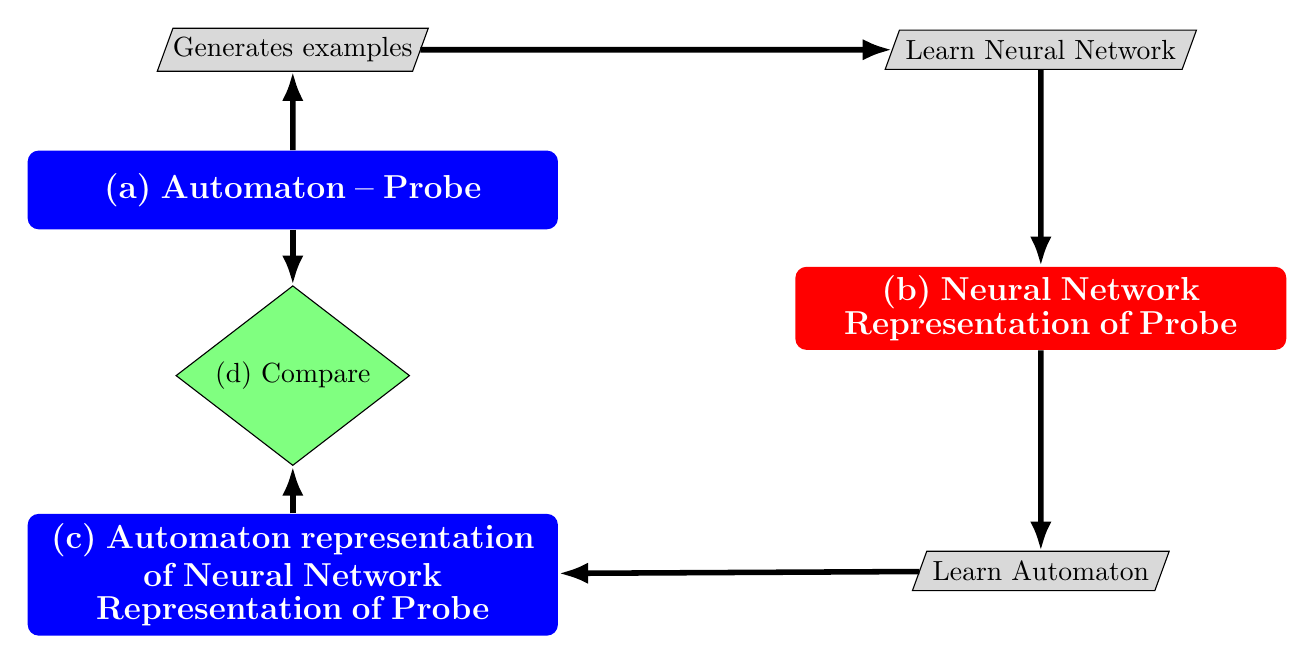
\begin{tikzpicture}[node distance=9.5cm]
				\node (start) [dfa] {\large \bf (a) Automaton -- Probe};
				\node (examples) [process, above = 1cm of start] {Generates examples};
				\node (learn1) [process, right of = examples] {Learn Neural Network};
				\node (step2) [nn, below= 2.5cm of learn1] {\large \bf (b) Neural Network \\ Representation of Probe};
				\node (end) [dfa, below = 3.6cm of start] {\large \bf  (c) Automaton representation \\ of Neural Network \\ Representation of Probe};
				\node (learn2) [process, below = 2.55 of step2] {Learn Automaton};
				\node (compare) [comparison, above = 0.6cm of end] {(d) Compare};
				\draw [FARROW] (start) -- (examples);
				\draw [FARROW] (examples) -- (learn1);
				\draw [FARROW] (learn1) -- (step2);
				\draw [FARROW] (step2) -- (learn2);
				\draw [FARROW] (learn2) -- (end);
				\draw [FARROW] (end) -- (compare);
				\draw [FARROW] (start) -- (compare);
			\end{tikzpicture}
		\end{center}
		\caption{Learning and testing strategy}
		\label{diag:strategy}
	\end{figure}
	
	\bibliographystyle{plain}
	\bibliography{references}
	
\end{document}